% Options for packages loaded elsewhere
\PassOptionsToPackage{unicode}{hyperref}
\PassOptionsToPackage{hyphens}{url}
%
\documentclass[
]{article}
\title{Patterns of Adolescent Physical Activity}
\author{Elizabeth Bates, Esmeralda Castro, \& Zach Farley}
\date{12/8/2021}

\usepackage{amsmath,amssymb}
\usepackage{lmodern}
\usepackage{iftex}
\ifPDFTeX
  \usepackage[T1]{fontenc}
  \usepackage[utf8]{inputenc}
  \usepackage{textcomp} % provide euro and other symbols
\else % if luatex or xetex
  \usepackage{unicode-math}
  \defaultfontfeatures{Scale=MatchLowercase}
  \defaultfontfeatures[\rmfamily]{Ligatures=TeX,Scale=1}
\fi
% Use upquote if available, for straight quotes in verbatim environments
\IfFileExists{upquote.sty}{\usepackage{upquote}}{}
\IfFileExists{microtype.sty}{% use microtype if available
  \usepackage[]{microtype}
  \UseMicrotypeSet[protrusion]{basicmath} % disable protrusion for tt fonts
}{}
\makeatletter
\@ifundefined{KOMAClassName}{% if non-KOMA class
  \IfFileExists{parskip.sty}{%
    \usepackage{parskip}
  }{% else
    \setlength{\parindent}{0pt}
    \setlength{\parskip}{6pt plus 2pt minus 1pt}}
}{% if KOMA class
  \KOMAoptions{parskip=half}}
\makeatother
\usepackage{xcolor}
\IfFileExists{xurl.sty}{\usepackage{xurl}}{} % add URL line breaks if available
\IfFileExists{bookmark.sty}{\usepackage{bookmark}}{\usepackage{hyperref}}
\hypersetup{
  pdftitle={Patterns of Adolescent Physical Activity},
  pdfauthor={Elizabeth Bates, Esmeralda Castro, \& Zach Farley},
  hidelinks,
  pdfcreator={LaTeX via pandoc}}
\urlstyle{same} % disable monospaced font for URLs
\usepackage[margin=1in]{geometry}
\usepackage{graphicx}
\makeatletter
\def\maxwidth{\ifdim\Gin@nat@width>\linewidth\linewidth\else\Gin@nat@width\fi}
\def\maxheight{\ifdim\Gin@nat@height>\textheight\textheight\else\Gin@nat@height\fi}
\makeatother
% Scale images if necessary, so that they will not overflow the page
% margins by default, and it is still possible to overwrite the defaults
% using explicit options in \includegraphics[width, height, ...]{}
\setkeys{Gin}{width=\maxwidth,height=\maxheight,keepaspectratio}
% Set default figure placement to htbp
\makeatletter
\def\fps@figure{htbp}
\makeatother
\setlength{\emergencystretch}{3em} % prevent overfull lines
\providecommand{\tightlist}{%
  \setlength{\itemsep}{0pt}\setlength{\parskip}{0pt}}
\setcounter{secnumdepth}{-\maxdimen} % remove section numbering
\newlength{\cslhangindent}
\setlength{\cslhangindent}{1.5em}
\newlength{\csllabelwidth}
\setlength{\csllabelwidth}{3em}
\newlength{\cslentryspacingunit} % times entry-spacing
\setlength{\cslentryspacingunit}{\parskip}
\newenvironment{CSLReferences}[2] % #1 hanging-ident, #2 entry spacing
 {% don't indent paragraphs
  \setlength{\parindent}{0pt}
  % turn on hanging indent if param 1 is 1
  \ifodd #1
  \let\oldpar\par
  \def\par{\hangindent=\cslhangindent\oldpar}
  \fi
  % set entry spacing
  \setlength{\parskip}{#2\cslentryspacingunit}
 }%
 {}
\usepackage{calc}
\newcommand{\CSLBlock}[1]{#1\hfill\break}
\newcommand{\CSLLeftMargin}[1]{\parbox[t]{\csllabelwidth}{#1}}
\newcommand{\CSLRightInline}[1]{\parbox[t]{\linewidth - \csllabelwidth}{#1}\break}
\newcommand{\CSLIndent}[1]{\hspace{\cslhangindent}#1}
\usepackage{amsmath}
\usepackage{booktabs}
\usepackage{caption}
\usepackage{longtable}
\ifLuaTeX
  \usepackage{selnolig}  % disable illegal ligatures
\fi

\begin{document}
\maketitle

Liz: - Write 3rd paragraph in intro - Methods Section (minus esmes part)
- Start results section with in-text code (N = , \% boys/girls, avg age,
avg weekly MVPA) to describe summary table, and insert summary table. -
Data analysis section (short paragraph) Esme: - Data analysis portion -
Inserting figures/code chunks where needed - Discussion Section Zach: -
Write 2 Intro paragraphs (done) - Preliminary methods sections (done) -
Abstract (after everyone else is done) - Make bibliography - In text
citations - Final Formatting

\hypertarget{abstract}{%
\section{Abstract}\label{abstract}}

\textbf{ZACH WILL WRITE AT THE END}

\hypertarget{introduction}{%
\section{Introduction}\label{introduction}}

It is well known that regular physical activity (PA) is associated with
a myriad of physical and mental health benefits. These benefits may be
proximal in time to the performance of PA, such as reduced anxiety-like
feelings, lower blood pressure, and enhanced cognitive function, or they
may be more distal, such as increased strength and cardio-respiratory
fitness, decreased depression-like symptoms, and long-term reduction of
blood pressure \emph{(Piercy KL, Troiano RP, Ballard RM, et al.~The
Physical Activity Guidelines for Americans. JAMA.
2018;320(19):2020--2028. \url{doi:10.1001/jama.2018.14854)_}. Regular PA
is especially important for school-aged children (6-17 years old); PA
has been shown to foster normal growth and development, improve mood and
sleep quality, and greatly reduce the risk for developing chronic
disease(s) as an adult }(Piercy KL, Troiano RP, Ballard RM, et al.~The
Physical Activity Guidelines for Americans. JAMA.
2018;320(19):2020--2028. \url{doi:10.1001/jama.2018.14854}).\_ Aside
from these physiological benefits, physically active students tend to
have better educational outcomes (e.g., better grades, enhanced
cognitive performance, and decreased behavioral problems) when compared
to their less-active peers \emph{(Centers for Disease Control and
Prevention. The Association Between School-Based Physical Activity,
Including Physical Education, and Academic Performance. Atlanta, GA;
Centers for Disease Control and Prevention, US Department of Health and
Human Services; 2010.).} As outlined by the U.S. Department of Health
and Human Services 2nd edition of the ``Physical Activity Guidelines for
Americans'' (2018), the recommended daily dose of moderate- to
vigorous-intensity physical activity (MVPA) for school-aged youth in the
United States (US) is 60 minutes \emph{(CITE
\url{https://health.gov/our-work/nutrition-physical-activity/physical-activity-guidelines/current-guidelines)_}.
Despite these recommendations the benefits of meeting them, less than a
quarter (24\%) of school-aged children in the US achieve the recommended
60 minutes of MVPA a day }(The Child \& Adolescent Health Measurement
Initiative (CAHMI). 2016 National Survey of Childrens Health. Data
Resource Center for Child and Adolescent Health;2016).\_ \textbf{need to
remove the citations that were removed from the intro I started} NEED
ANOTHER PARAGRAPH THAT TOUCHES ON THE SPECIFICS IN THE LITERATURE
ASSOCIATED WITH OUR RESEARCH QUESTIONS, TO LEAD INTO STATING OUR RQs.

\hypertarget{research-questions}{%
\subsection{Research Questions}\label{research-questions}}

\textbf{1. How do patterns of physical activity for adolescents vary by
sex after controlling for age and BMI?}

\textbf{2. Does minutes of physical activity performed during the week
differ by the type of school attended (private, public, home, or other)
}

\hypertarget{hypotheses}{%
\subsection{Hypotheses}\label{hypotheses}}

\textbf{1. Patterns of physical activity of adolescents will
significantly vary by sex after controlling for age and BMI.}

\textbf{2. There will be a significant association between the type of
school attended at the weekday minutes of physical activity performed by
adolescents.}

\hypertarget{methods}{%
\section{Methods}\label{methods}}

\hypertarget{data-source}{%
\subsection{Data Source}\label{data-source}}

This project uses data from the Family Life, Activity, Sun, Health and
Eating (FLASHE) study. FLASHE data was collected through a
cross-sectional design, using an internet-based survey \emph{(CITE from
\url{https://cancercontrol.cancer.gov/brp/hbrb/flashe-study}).}\textbf{Zach,
I think you should cite the Oh 2017 article (in .bib file) for previous
sentence}. Data collection occurred between April and October of 2014.
The FLASHE study asked questions enabling researchers to examine
correlates of cancer-related behaviors using behavioral measures of diet
and physical activity, and other behaviors associated with cancer risk,
such as sun-safety, sleep, and tobacco consumption. Sampling for the
FLASHE study was drawn from a Consumer Opinion Panel and sampling design
was intended to collect a representative sample reflective of
demographics for the United States' general population (e.g., sex,
education, income, age, region, household size). The conceptual model
for the FLASHE study can be seen in Figure 1. It is important to note
that data collection took place by sampling dyads of
parent/caregiver-adolescent(ages 12-17). The FLASHE enrollment and
design structure can be seen in Figure 2.

\hypertarget{figure-1-flashe-conceptual-model}{%
\subsubsection{Figure 1: FLASHE Conceptual
Model}\label{figure-1-flashe-conceptual-model}}

\begin{figure}
\centering
\includegraphics{/Users/zsfarley/Desktop/images/FLASHE_Concept.jpg}
\caption{FLASHE Conceptual Model}
\end{figure}

\hypertarget{figure-2-flashe-enrollment-and-design}{%
\subsubsection{Figure 2: FLASHE Enrollment and
Design}\label{figure-2-flashe-enrollment-and-design}}

\begin{figure}
\centering
\includegraphics{/Users/zsfarley/Desktop/images/FLASHE_Enrollment.jpg}
\caption{FLASHE Enrollment and Design}
\end{figure}

\hypertarget{sample-selection}{%
\subsection{Sample Selection}\label{sample-selection}}

In our study, we aim to examine patterns of adolescent \textbf{isn't
this MVPA?-\textgreater{}}PA, including when and how much \textbf{same
here}PA they perform, and to explore the association between
adolescents' weekly minutes of MVPA and their sex, after adjusting for
age and BMI as well as explore the association between adolescent's
school type with their exercise patterns. For the purpose of this study,
our final sample will be composed of teenagers (13-17 years old) who
gave responses for all physical activity and demographic variables. This
process and final sample size is explained in the following sections.

\hypertarget{statistical-analysis}{%
\subsection{Statistical Analysis}\label{statistical-analysis}}

\emph{Demographic Characteristics} Descriptive statistics were performed
to determine the distribution of study variables among participants and
to check for skewness and kurtosis. All analysis was conducted with the
statistical software R (R Core Team 2021).

\hypertarget{calculating-bmi---mutate}{%
\subsubsection{Calculating BMI -
\{mutate\}}\label{calculating-bmi---mutate}}

Body Mass Index (BMI) is an effective measure of \_\_\_\_\_(Esme and
Zach this is your wheel house, so leaving this definition and noting
importance of BMI to you :) To calculate BMI, we utilized the \{mutate\}
function.

\hypertarget{joining-data-sets-not-in-paper-but-move-to-other-rmd-file}{%
\subsubsection{Joining Data Sets (NOT IN PAPER BUT MOVE TO OTHER RMD
FILE)}\label{joining-data-sets-not-in-paper-but-move-to-other-rmd-file}}

\emph{Our data was split into two files for size/downloadable reasons:
adolescent demographic and adolescent physical activity surveys. Each of
these files contained a column containing the variable ``PID,'' or
participant identification. The PIDs are unique to each individual who
completed the surveys. We used this variable to join these two data
sets. This was done using the full join function from the dplyr package.
(CITE DPLYR PACKAGE) This was used so we could retain all variables
contained within both data sets for each specific participant identified
by their unique PID. After fully joining these two data sets, we then
needed to tidy up data using functions from the tidyverse and dplyr
packages (cite tidyverse and dplyr).}

\emph{(Load \& Join Data Sets Code CHUNK)}

\hypertarget{cleaning-data---select-characterize-and-filter-not-in-paper-but-move-to-other-rmd-file}{%
\subsubsection{Cleaning data - \{select\}, \{characterize\}, and
\{filter\} (NOT IN PAPER BUT MOVE TO OTHER RMD
FILE)}\label{cleaning-data---select-characterize-and-filter-not-in-paper-but-move-to-other-rmd-file}}

\emph{We then wanted to characterize only select variables, hence the
use of the \{select\}--\textgreater{} \{characterize\} functions. We
could not find a way to characterize the data set as a whole without
turning some variables' values to NA, so we selected certain variables,
characterized them, then rejoined the data sets with the newly
characterized data.}

\emph{(Cleaning Code Chunks)}

\hypertarget{calculating-mean-physical-activity---summarize-and-group_by}{%
\subsubsection{Calculating Mean Physical Activity - \{summarize\} and
\{group\_by\}}\label{calculating-mean-physical-activity---summarize-and-group_by}}

\emph{The \{group\_by\} function allowed us to organize our data by
school type and sex to appropriately assess for associations between
those demographic variables and average total weekly physical activity.}

\hypertarget{pivot_longer-for-organzing-when-physical-activity-occurs}{%
\subsubsection{\{pivot\_Longer\} for organzing when physical activity
occurs}\label{pivot_longer-for-organzing-when-physical-activity-occurs}}

\emph{The initial data set divided when physical activity was completed
by during the week in school (XTPREDWEEKS), during the week out of
school (XTPREDWEEKOFS), and on the weekend(XTPREDWEEKW). Using
\{pivot\_longer\}, we combined the variables of when/where the physical
activity was completed to better visualize across the pattern of
when/where and any associations with demographic variables.}

\hypertarget{results}{%
\section{Results}\label{results}}

Add in-text code showing mean bmi, age distribution, school-type \%s,
average weekly mvpa.

\hypertarget{summary-table}{%
\subsection{Summary Table}\label{summary-table}}

\captionsetup[table]{labelformat=empty,skip=1pt}
\begin{longtable}{lc}
\caption*{
{\large Table 1. Descriptive Characteristics}
} \\ 
\toprule
\textbf{Characteristic} & \textbf{N = 1,192}\textsuperscript{1} \\ 
\midrule
Sex &  \\ 
Female & 599 (50\%) \\ 
Male & 593 (50\%) \\ 
School Type &  \\ 
Another kind of school & 18 (1.5\%) \\ 
Home-schooled & 65 (5.5\%) \\ 
Private school & 84 (7.0\%) \\ 
Public school & 1,025 (86\%) \\ 
Race/Ethnicity &  \\ 
Hispanic & 127 (11\%) \\ 
Non-hispanic Black alone & 195 (16\%) \\ 
Non-hispanic White alone & 775 (65\%) \\ 
Other & 95 (8.0\%) \\ 
Age &  \\ 
13 years old & 280 (23\%) \\ 
14 years old & 223 (19\%) \\ 
15 years old & 241 (20\%) \\ 
16 years old & 286 (24\%) \\ 
17 years old & 162 (14\%) \\ 
 \bottomrule
\end{longtable}
\vspace{-5mm}
\begin{minipage}{\linewidth}
\textsuperscript{1}n (\%) \\ 
\end{minipage}

\newpage

\hypertarget{references}{%
\section{References}\label{references}}

have code for the summary table in script and can turn it into a plot
like bar/col or error bars \#\# MVPA by Demographic Variables
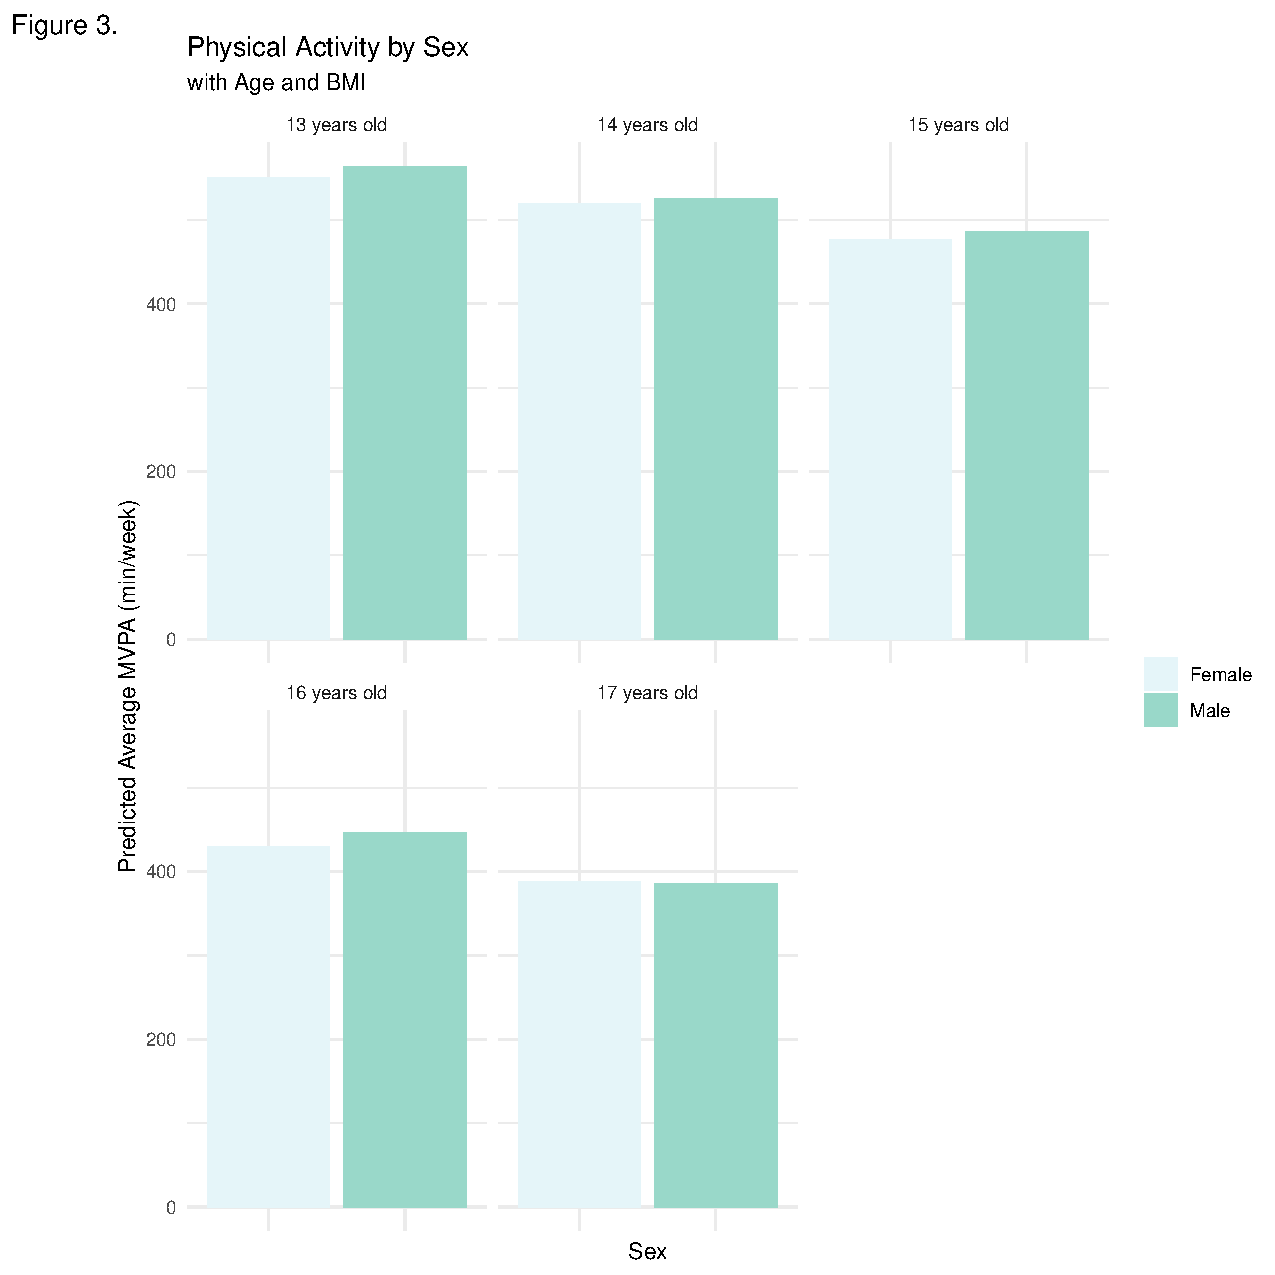
\includegraphics{FLASHEPaper_files/figure-latex/PA-BMI-race-ethnicity-1.pdf}

\hypertarget{mvpa-by-school-type}{%
\subsection{MVPA by School Type}\label{mvpa-by-school-type}}

\includegraphics{FLASHEPaper_files/figure-latex/PA-by-school-type-1.pdf}

\hypertarget{figure-3}{%
\subsection{Figure 3}\label{figure-3}}

\hypertarget{discussion}{%
\section{Discussion}\label{discussion}}

Based on our analysis of adolescents who participated in the FLASE
study\ldots{} Implications for programs to promote physical activity in
or out of school.. Implications for policy.. Next steps for research
include examining what motivates adolescents to complete physical
activity, and how their environment moderates or mediates the amount of
physical activity they complete.

Note that the \texttt{echo\ =\ FALSE} parameter was added to the code
chunk to prevent printing of the R code that generated the plot.

\newpage

\hypertarget{references-1}{%
\section{References}\label{references-1}}

\textbf{note I cannot correctly format US Dept of HHS}

\hypertarget{refs}{}
\begin{CSLReferences}{1}{0}
\leavevmode\vadjust pre{\hypertarget{ref-R}{}}%
R Core Team. 2021. \emph{R: A Language and Environment for Statistical
Computing}. Vienna, Austria: R Foundation for Statistical Computing.
\url{https://www.R-project.org/}.

\end{CSLReferences}

\end{document}
